\subsection{Introduction}

\label{sec:kpimm:introduction}

The decay \BdToKpimm is a flavour-changing neutral-current process. In the Standard Model (SM), the leading order transition amplitudes are described by electroweak penguin or box diagrams.  In extensions to the SM, new heavy particles can contribute to loop diagrams and modify observables such as branching fractions and angular distributions.

\subsubsection[Previous \btosmm measurements]{Previous \boldmath{\btosmm} measurements}
The previous angular analyses of \BdToKpimm performed by the \lhcb collaboration~\cite{LHCB-PAPER-2011-020,LHCB-PAPER-2013-019,LHCB-PAPER-2013-037,LHCB-PAPER-2015-051} focused on the $K^{+}\pi^{-}$ invariant mass range $796<\mkpi<996\mevcc$ where the decay proceeds predominantly via the P-wave process $\decay{\Kstar(892)^{0}}{\kpi}$. A global analysis of the \CP-averaged angular observables measured in the \lhcb Run 1 data sample indicated differences with SM predictions at the level of 3.4 standard deviations~\cite{LHCB-PAPER-2015-051}. The results of the measurement of the observable $P_{5}^{'}$, which exhibits a local deviation from the SM predictions, is shown in Fig.~\ref{fig:kpimm:p5prime}.

\begin{figure}[!b]
\centering
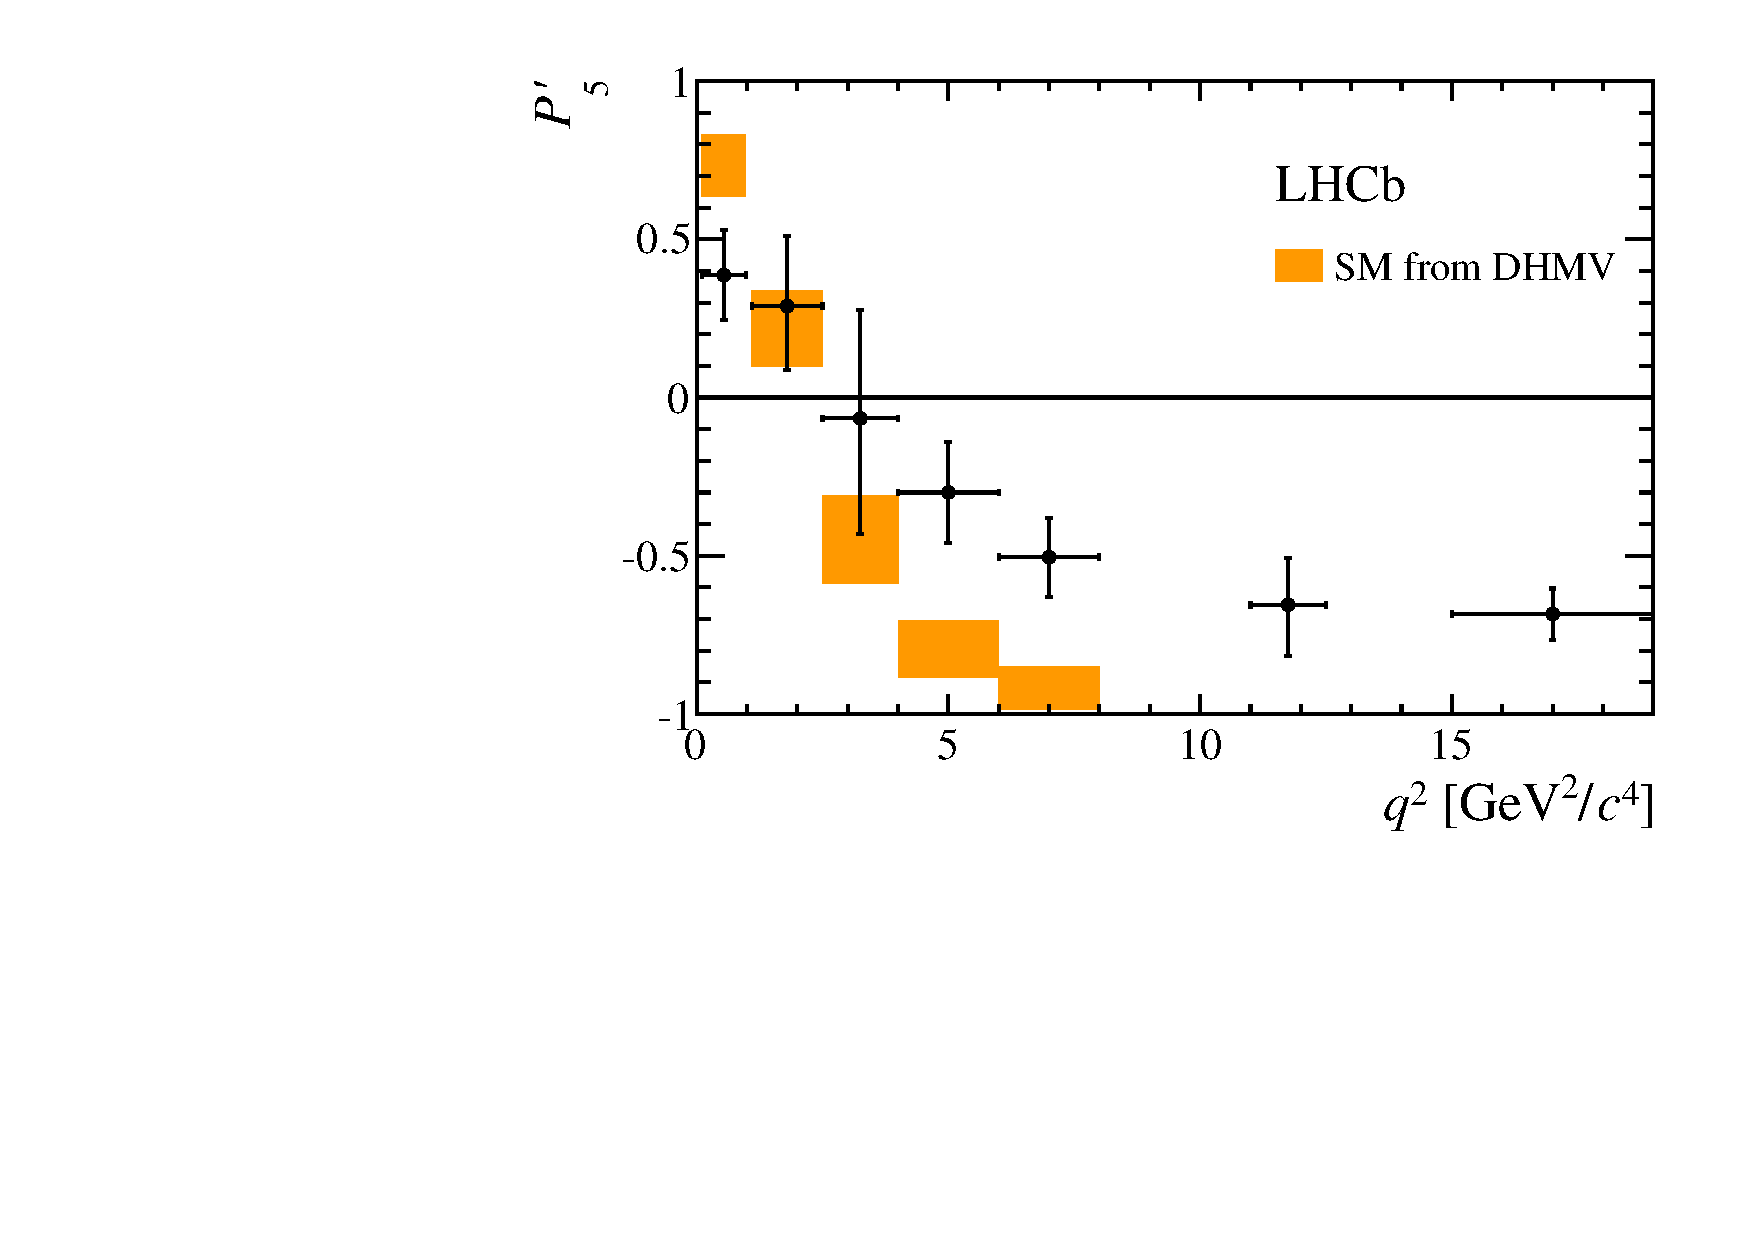
\includegraphics[width=0.7\textwidth]{figs/kpimm/introduction/P5prime.pdf}
\caption{Results of the measurement of the observable $P_{5}^{'}$ by the \lhcb collaboration. The SM predictions are taken from Ref.~\cite{pprime-theory}.}
\label{fig:kpimm:p5prime}
\end{figure}

This set of measurements is part of a pattern of discrepancies with respect to SM predictions that have been observed in \btosmm transitions. For example, the measured differential branching fractions of the decays \BsTophimm~\cite{LHCB-PAPER-2015-023}, $\decay{\Lb}{\Lambda\mumu}$~\cite{LHCB-PAPER-2015-009} and \BuToKmm~\cite{LHCB-PAPER-2014-006} all lie below their corresponding SM predictions. Furthermore, the ratio $R_{K} = \BF(\decay{\Bp}{\Kp\mup\mun})/\BF(\decay{\Bp}{\Kp\ep\en})$, which is a test of lepton flavour universality, was also measured to be 2.6 standard deviations from its SM prediction of unity~\cite{LHCB-PAPER-2014-024}.

This pattern of discrepancies can be intepreted by performing global model-independent fits to \btosmm measurements~\cite{Altmannshofer:2015sma}.{\interfootnotelinepenalty=10000\footnote{The global fit in Ref.~\cite{Altmannshofer:2015sma} takes into account 88 measurements of 76 observables by the \atlas, \babar, \belle, \cdf, \cms and \lhcb experiments.}} In the framework of OPE, described in Sec~\ref{sec:theory:rare}, these fits can be used to constrain the values of the Wilson coefficients $\mathcal{C}_{7}$, $\mathcal{C}_{9}$ and $\mathcal{C}_{10}$. A $\chi^{2}$ function which quantifies the compatibility of the model with the data, for a given set of values of the Wilson coefficients, is minimised in different scenarios. The NP dependencies are encoded as NP contributions to the Wilson coefficients, $\mathcal{C}_{i}^{\rm NP} = \mathcal{C}_{i}-\mathcal{C}_{i}^{\rm SM}$. The best fit is obtained when allowing NP in $\mathcal{C}_{9}$ only, yielding a value of $\mathcal{C}_{9}^{\rm NP} = -1.07$ which correponds to a pull of 3.7 standard deviations from the SM. Figure~\ref{fig:kpimm:c9c10} shows the result of the fit when allowing for NP effects in both $\mathcal{C}_{9}$ and $\mathcal{C}_{10}$. These results are in good agreement with Ref.~\cite{Descotes-Genon:2015uva}, which also finds that a negative contribution to $\mathcal{C}_{9}$ plays a central role in explaining the observed discrepancies.

\begin{figure}[!tb]
\centering
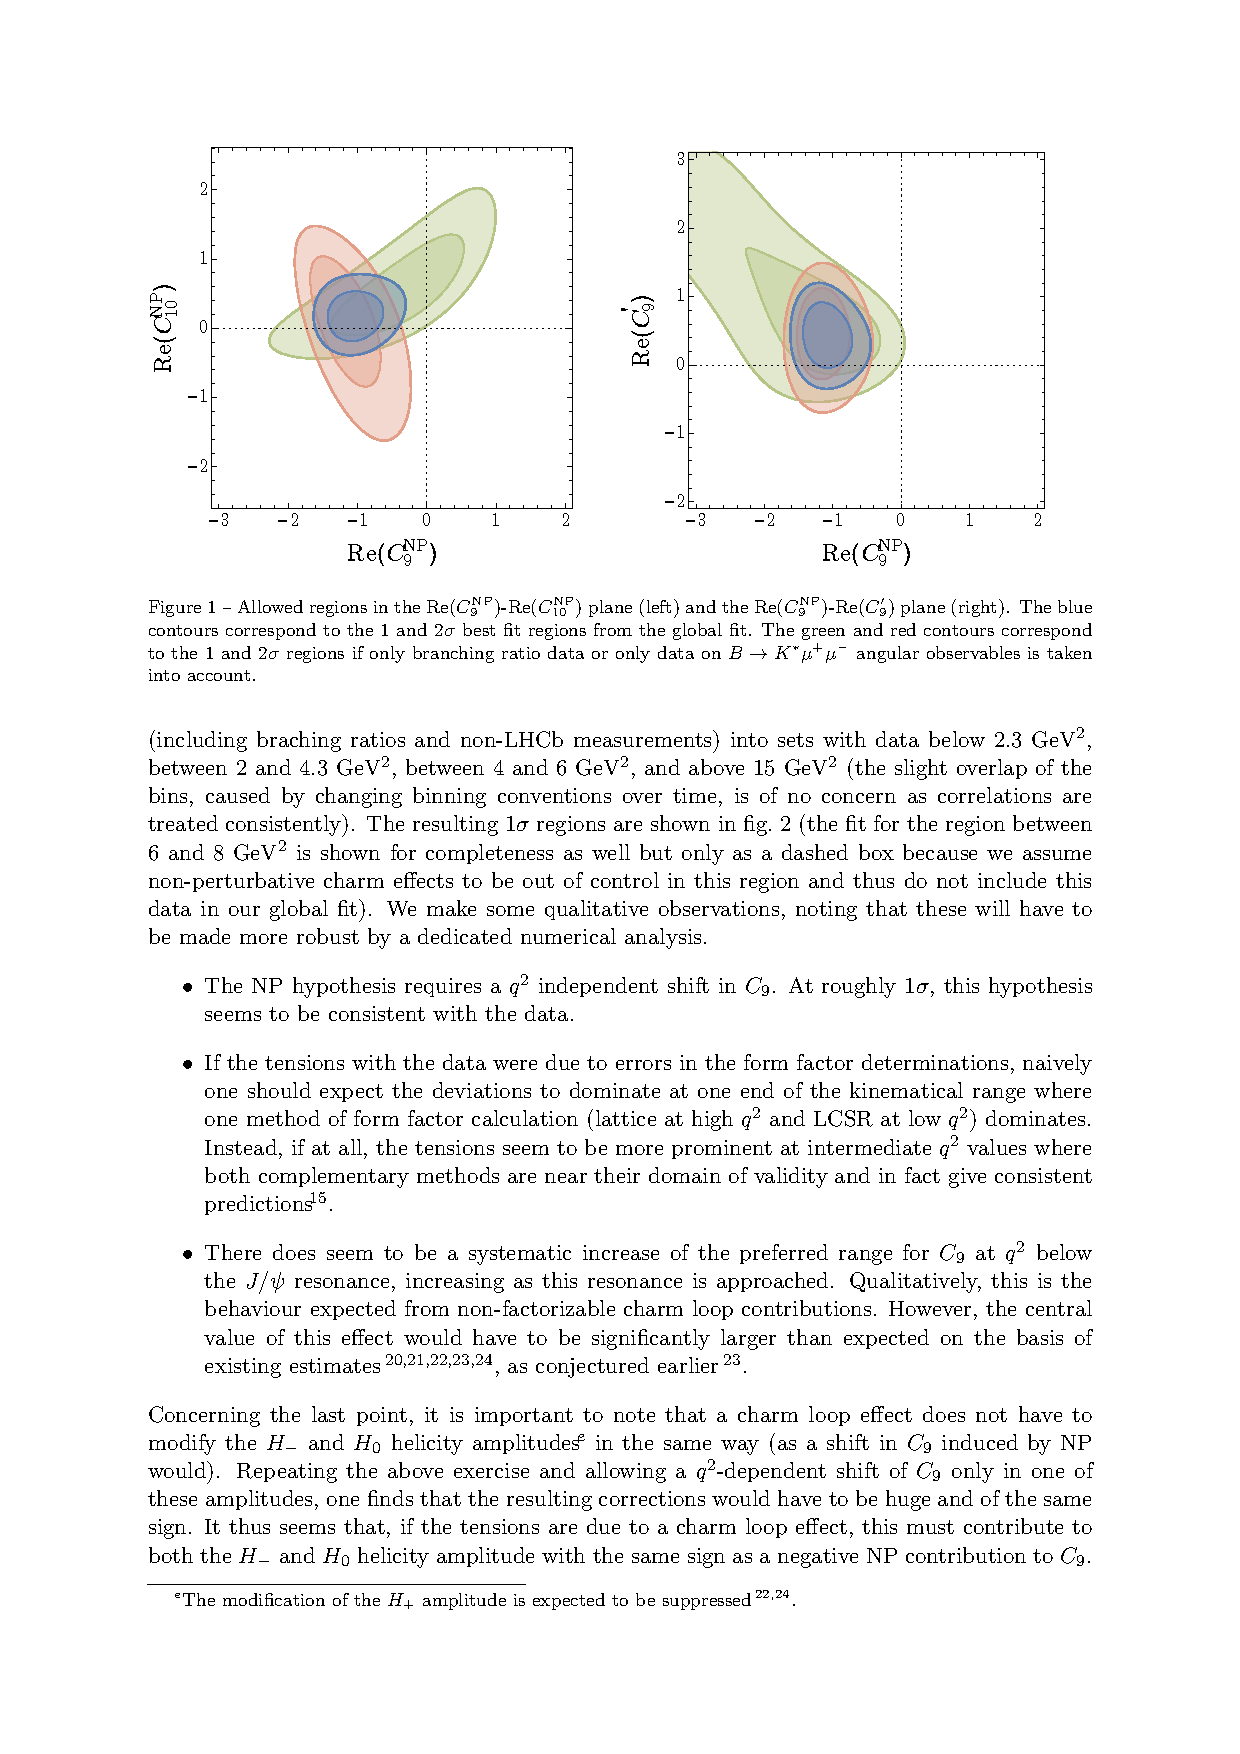
\includegraphics[trim={2.5cm 20cm 10.7cm 2.4cm},clip,width=0.6\textwidth]{figs/kpimm/introduction/c9c10.pdf}
\caption{Allowed region in the ${\rm Re}(\mathcal{C}_{9}^{\rm NP})$--${\rm Re}(\mathcal{C}_{10}^{\rm NP})$ plane. The blue contours correspond to the 1$\sigma$ and 2$\sigma$ best fit regions from the global fit. The red and green contours represent 1$\sigma$ and 2$\sigma$ regions if only the \BdToKstmmP angular observables or only the differential branching fraction measurements are taken into account, respectively. Taken from Ref.~\cite{Altmannshofer:2015sma}.}
\label{fig:kpimm:c9c10}
\end{figure}

Many NP models have been proposed to explain this observed tension from the SM in $\mathcal{C}_{9}$. Such models contain new interactions mediated by a $Z^{'}$ boson~\cite{Gauld:2013qja,Altmannshofer:2014cfa,Crivellin:2015mga} or leptoquarks~\cite{Sahoo:2015wya,Biswas:2014gga,Hiller:2014ula}. These interactions can also introduce a violation of lepton flavour universality.

However, it has also been suggested that the contribution of so-called charm-loop effects could be responsible for the observed deviations~\cite{Lyon:2014hpa}. As these hadronic effects are mediated via virtual photon exchange, leading to a vector-like coupling to leptons, it is possible they could mimic NP effects in $\mathcal{C}_{9}$.

Since short distance effects are universal and should appear coherently in all \btosmm transitions, measuring other \btosmm transitions can help to shed light on this situation.

% \begin{figure}[!tb]
% \centering
% 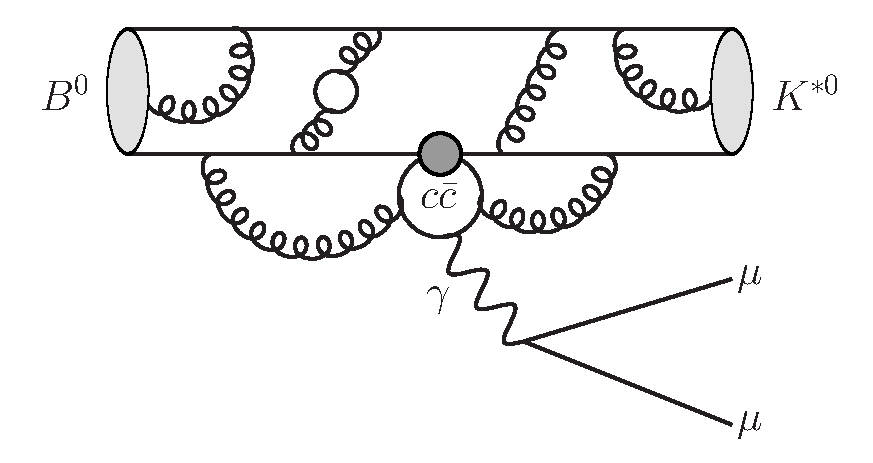
\includegraphics[width=0.6\textwidth]{figs/kpimm/introduction/btosll_charm.eps}
% \caption{}
% \label{fig:kpimm:charm-loops}
% \end{figure}

\subsubsection{Analysis overview}

Since the dominant structures in the \kpi invariant mass spectrum of \BdToKpimm above the P-wave $\Kstar(892)^{0}$ are resonances in the 1430\mevcc region, this is a natural region to study. The relevant \Kstarz states above the \KstP mass range are listed in Table~\ref{tab:introduction:states}. Throughout this paper, the symbol $\Kstarz$ denotes any neutral strange meson in an excited state that decays to a \Kp\pim final state. In the 1430\mevcc region, contributions are expected from the S-wave $K^\ast_0(1430)^0$, P-wave $K^\ast(1410)^0$ and D-wave $K^\ast_2(1430)^0$ states, as well as the broad P-wave $K^\ast(1680)^0$ state. 

\begin{table}[!tb]
\caption{Expected resonant contributions above the \KstP mass range. For each, the spin-parity, $J^P$, and branching fraction to $\kaon\pion$, $\mathcal{B}(K\pi)$, are given. Taken from Ref.~\cite{lu-wang}.}
\label{tab:introduction:states}
\centering
\begin{tabular}{c|c|c|c|r}
    Resonance & $J^{P}$ & Mass [$\mathrm{Me\kern -0.1em V\!/}c^2$] & Full width [$\mathrm{Me\kern -0.1em V\!/}c^2$]  & $\mathcal{B}(K\pi)~[\%]$ \\
   \hline
   $K^\ast(1410)^0$ & $1^{-}$& $\hphantom{0.}1414 \pm 15\hphantom{.}$& $232 \pm 21\hphantom{0}$  & $6.6 \pm 1.3$ \\
   $K^\ast_0(1430)^0$ & $0^{+}$ & $\hphantom{0.}1425 \pm 50\hphantom{.}$ & $270 \pm 80\hphantom{0}$ & $\hphantom{.}93 \pm 10\hphantom{.}$ \\
   $K^\ast_2(1430)^0$ & $2^{+}$ & $1432.4\pm 1.3$ & $109 \pm 5\hphantom{00}$ & $49.9 \pm 1.2$ \\
   $K^\ast(1680)^0$ & $1^{-}$ & $\hphantom{0.}1717 \pm 27\hphantom{.}$ & $322 \pm 110$ & $38.7 \pm 2.5$ \\
   $K^\ast_3(1780)^0$ & $3^{-}$ & $\hphantom{0.}1776 \pm 7\hphantom{0.}$ & $159 \pm 21\hphantom{0}$ & $18.8 \pm 1.0$ \\
   $K^\ast_4(2045)^0$ & $4^{+}$ & $\hphantom{0.}2045 \pm 9\hphantom{0.}$ & $198 \pm 30\hphantom{0}$ & $9.9 \pm 1.2$ \\
 \end{tabular}
 \end{table}

The \mkpi distribution for \BdToKpimm decays in the range $1.1<\qsq<6.0\gevgevcccc$ and $630<\mkpi<1630\mevcc$ is shown in Fig.~\ref{fig:full-mkpi}, where $\qsq \equiv m^2(\mup \mun)$. The candidates are obtained using the selection described in Sec.~\ref{sec:kpimm:selection} and the background component is subtracted using the \sPlot technique~\cite{splot}. The main structures are observed around the mass of the $\Kstar(892)^{0}$ resonance and in the 1430\mevcc region. 

\begin{figure}[!tb]
 \centering
 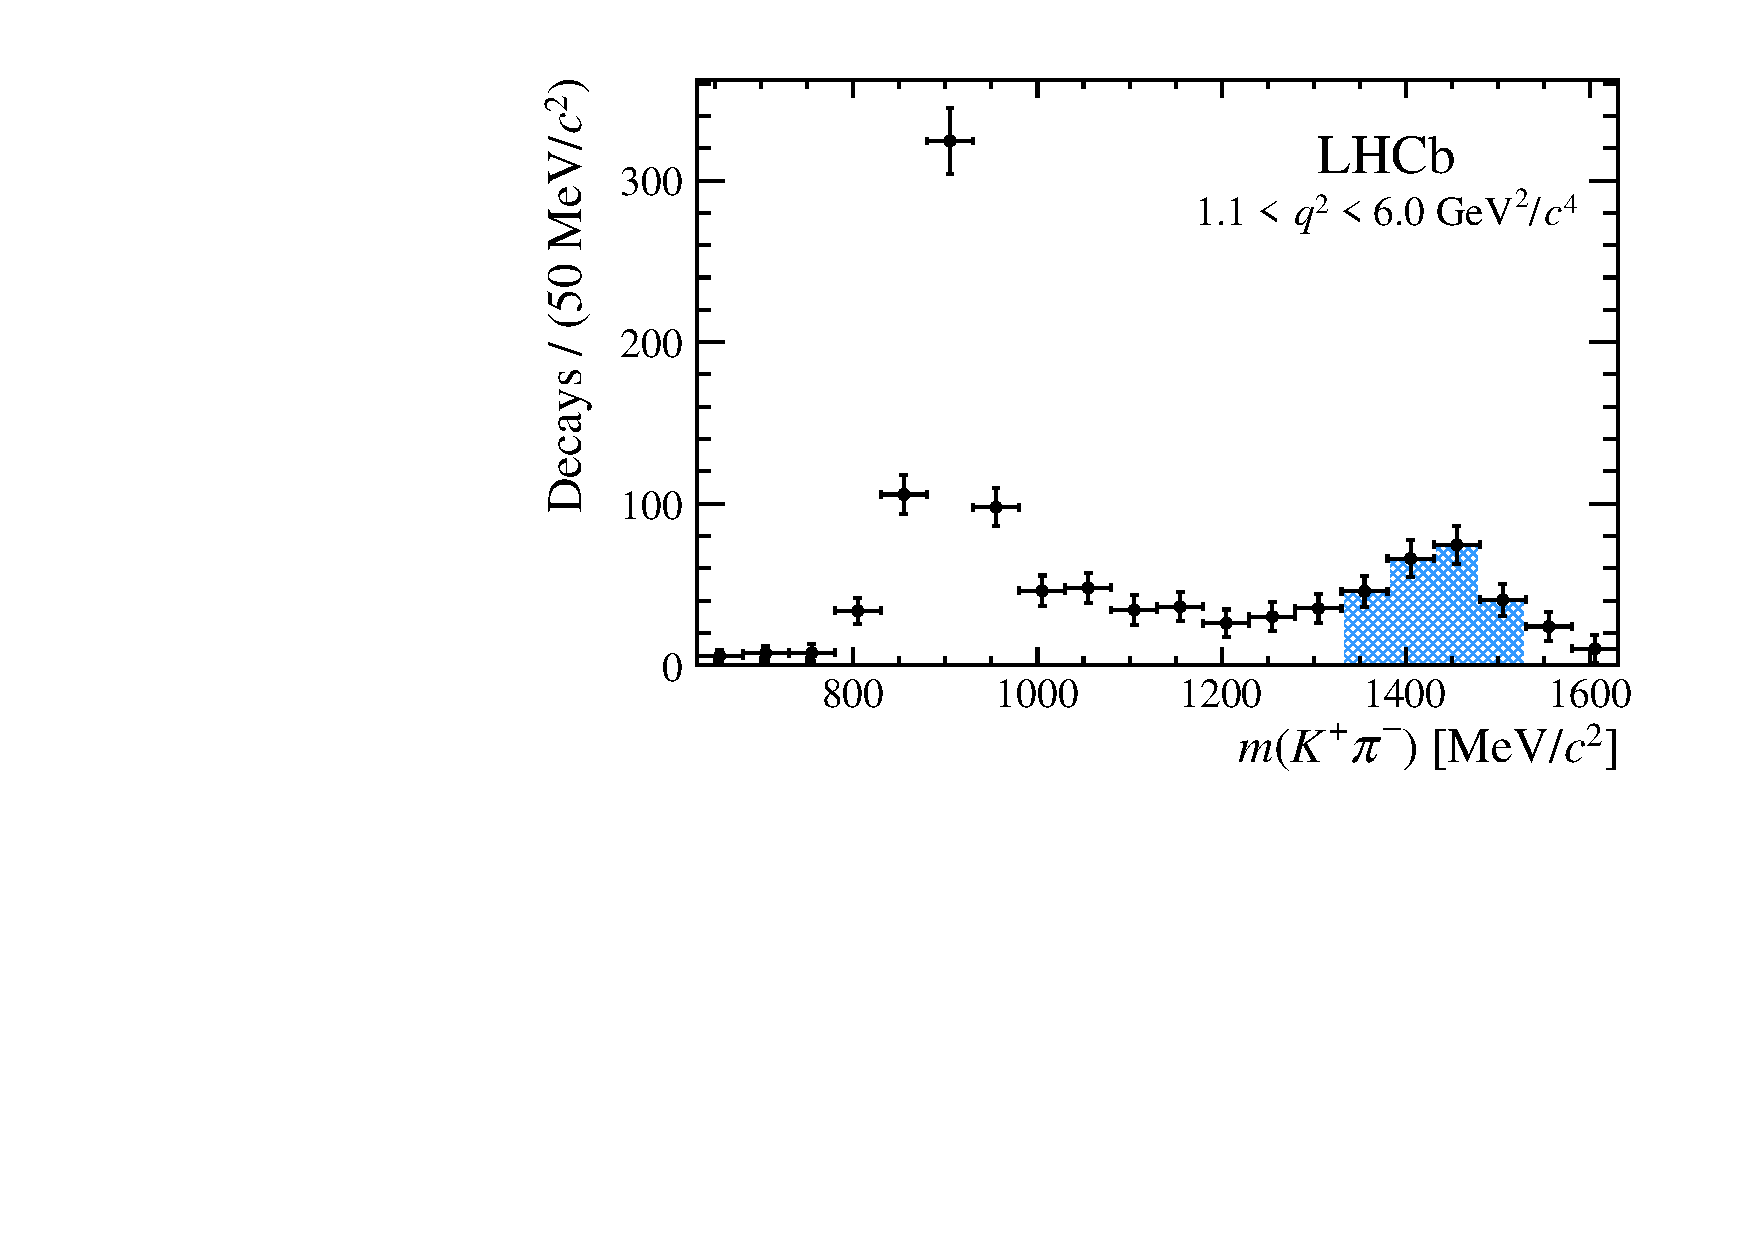
\includegraphics[width=0.7\linewidth]{figs/kpimm/introduction/full-mkpi.pdf}
 \caption{Background-subtracted \mkpi distribution for \BdToKpimm decays in the range $1.1<\qsq<6.0\gevgevcccc$. The region $1330<\mkpi<1530~\mevcc$ is indicated by the blue hatched area.}
\label{fig:full-mkpi}
\end{figure}

This chapter describes the first measurements of the differential branching fraction and angular moments of \BdToKpimm in the region $1330<\mkpi<1530\mevcc$. The values of the differential branching fraction are reported in five bins of \qsq between 0.1 and 8.0\gevgevcccc, and in the range $1.1<\qsq<6.0\gevgevcccc$ for which the angular moments are also measured. The measurements are based on samples of $pp$ collisions collected by the \lhcb experiment in Run 1, corresponding to integrated luminosities of 1.0\invfb at a centre-of-mass energy of 7\tev and 2.0\invfb at 8\tev.  